%pdflatex -synctex=1 -interaction=nonstopmode gemaDOc.tex

\documentclass[a4paper, 11pt]{article}
\usepackage{setspace}
\setstretch{1.5}
\usepackage[ngerman]{babel}
\usepackage[utf8]{inputenc}
\usepackage{graphicx}

%Eurozeichen: €
\usepackage{eurosym} 
%raender kleiner machen
\usepackage{geometry}
\geometry{verbose,a4paper,bottom=3cm}

%Fußnoten ohne Nummern
\usepackage{nccfoots}
%Klickbare Links
%\usepackage[hidelinks]{hyperref}
\usepackage[hyphens]{url}
\usepackage{hyperref}
\usepackage{xcolor}
\hypersetup{
    colorlinks,
    linkcolor={blue!40!black},
    citecolor={blue!50!black},
    urlcolor={blue!60!black}
}

%umlgraphics
%\ifx\pdftexversion\undefined
%\usepackage[dvips]{graphicx}
%\else
%\usepackage[pdftex]{graphicx}
\DeclareGraphicsRule{*}{mps}{*}{}
%\fi

\usepackage{helvet}
\renewcommand{\familydefault}{\sfdefault}

\pagestyle{myheadings}
\markright{HAW Hamburg, Media Systems, SoSe 15}
\begin{document}
\newpage


\begin{verbatim}




\end{verbatim}
\begin{center}


\newcommand{\HRule}{\rule{\linewidth}{0.5mm}}
\HRule \\[0.4cm]
{ \huge \bfseries Entwicklerhandbuch}
\HRule

\Large{Natural Beverages Webshop} \\[1cm]

\begin{minipage}{0.55\textwidth}
\begin{flushleft} \large
\emph{Author:} \\
\emph{Matrikelnummer:} \\
\emph{Fach:} \\
\emph{Dozent:}
\end{flushleft}
\end{minipage}
\hfill
\begin{minipage}{0.4\textwidth}
\begin{flushright} \large
\emph{Author \textsc{A}} \\
\emph{42} \\
\emph{RDB} \\
\emph{Dozent \textsc{A}}
\end{flushright}
\end{minipage}
\end{center}
\begin{verbatim}



\end{verbatim}

\begin{abstract}
\noindent %kein eingerueckter Satz
Ein Entwicklertagebuch zum RDB Projekt \\ [1cm]
\end{abstract}

\newpage

\tableofcontents
\listoffigures

\newpage
%fragestellung, Einleitung, Relevanz
\section{Einleitung - Konzept}
Natural Beverages ist ein Webshop der sich auf "natürliche" Getränke spezialisiert. Also Getränke aus Früchten, Getreide und anderen Rohstoffen. \\ 

Bio, FairTrade, lokale Ernährung sind aktuelle Stichworte und gerade zu Zeiten von Energy Drinks und Coca Cola hat sich eine Gruppe gefunden, die auf "natürliche" Produkte besteht. In diesem Sinne stellt "Natural Beverages" die Möglichkeit da auch lokale Sorten und Getränke zu kaufen. Hauptkategorien stellen Bier, Wein, Tees und Säfte.  
\section{Webseiten Design}

\subsection{Design}
Zum Darstellen der Elemente wird das CSS Framework Materialize (http://materializecss.com/about.html) genutzt. 

\subsection{Wege}
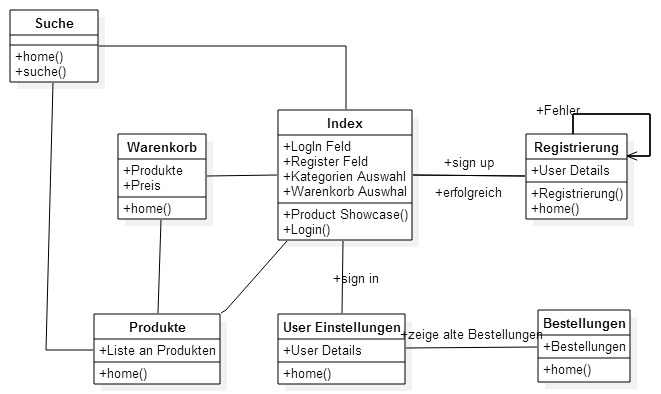
\includegraphics[width=\textwidth]{websiteWege.jpg}
\section{Programmtechnisches Design}

\subsection{Datenbank}
\includegraphics{databaseDesign.1}
Bei der Datenbank wurde stark auf den Verzicht von Id's geachtet. Id's machten letztendlich nur bei den Orders, sowie den Usern Sinn da, ein User am Tag mehrmals das gleiche bestellen kann und Date für einen Primary Key etwas unhandlich ist. Außerdem könnte sich die Email eines Users ändern. \\
Im Grunde teilt sich die Datenbank in drei Teile auf. Orders und Boughtgoods vereinigen dabei alle anderen: eine Bestellung eines Users enthällt gekaufte Produkte mit Anzahl und Preis welche wiederum auf das Produkt zugreifen. Produkt, Category, Crate und Container beschreiben damit das Produkt insgesamt mit allen Anteilen. \\
Es lässt sich darüber streiten ob ein solche Datenbankkonstrukt in der reellen Welt einsatzbereit ist. Sobald eine Kategorie umbenannt werden soll entsteht ein riesiger Schaden, da das nicht einfach so geschehen kann, ohne das Informationen verloren gehen können. Mit einer id als Primary Key wäre dies jedoch ohne weiteres möglich.

\subsection{Authentication und User Management}
Ein LogIn geschieht über einen Abruf und Abgleich der Datenbank. Das eingegebene Passwort wird in md5 gehasht und anschließen mit dem Datenbankeintrag (ebenfalls md5) abgeglichen. Vermutlich würde man in der reellen Welt eine bessere Hashingmethode verwenden. Beim erfolgreichen Einloggen wird der Session eine Variable("nick") gesetzt. \\
Ausloggen ist einfach nur das Entfernen dieser Variable.\\
Die Ursprüngliche Idee war einen Filter(siehe /WEB-INF/NaturalBeverages/SessionFilter.java) zu benutzen. Sofern die SessionVariable "nick" (die beim einloggen gesetzt wurde) nicht null beträgt, wird der Client auf die angeforderte Seite weiter- oder ansonsten auf eine Fehlerseite geführt. Problem daran ist, dass auf dem Produktionsserver (praxi) Annotations nicht funktionieren und die web.xml auch nicht anfassbar war. \\
Somit dient eine einfache Abfrage über jeder entsprechenden Seite zur Kontrolle der Authentikation.  

\subsection{Admin Tool}
Das "Admin Tool" ist ein auf Servlets basierendes Webtool mit dem sich Produkt Einträge aus der Datenbank hinzufügen und löschen lassen. Die Admintools werden durch den Zugriff auf /admin erreicht. 

\section{User Stories}
\begin{enumerate}
	\item As a client I want to browse the baverages of the shop
	\item As an older person I want the delivery service to carry my items into my apartment
	\item As a client I want to get a bill at the end of the order with the given address
		- I also want to see:
			- glass and crate refunds
			- delivery-into-apartment price per litre
	\item As a client I want to be able to find the beverages I am looking for
	\item As a client I want to be able to view a help page
	\item I want to have the comfort of a user account to store previous orders
	\end{enumerate}
\end{document}
